\subsection{Preprocessing}
\label{sec:preprocessing}

Our data was preprocessed so we obtain the following: A
space-efficient, performant, abstract level matching what we as humans
see. To actually get all those traits, we had to apply some tricks.
First, we need to establish the following: Remember that each level
may contain $30 \cdot 10^{6}$~entries at maximum~-- this requires
$30 \cdot 10^{6}\text{ bits} \div 8 = 3.75 \cdot 10^{6}\text{ bytes} =
3.75\text{ MB}$ (MB~are megabytes) of storage \emph{per level},
assuming we are able to compactly store eight entries per byte
(usually you need one byte per entry but as we have binary values, we
can store one value in one bit). With approximately 17\,000~levels, we
would then need
$3.75\text{ MB} \times 17\,000 \approx 63.75 \cdot 10^{3}\text{ MB} =
63.75\text{ GB}$ (GB~are gigabytes) of storage at maximum. While data
is cheap and this calculated number is the absolute maximum amount of
storage we may need, we would like our data to be more compact for
both efficiency and portability.

Even the data containing only layers of all tiles is so large that
keeping the full database in 8~gigabytes of memory is not
possible\footnote{This is the amount of unused RAM the author had
  available on his laptop while working with about 2\,000~browser tabs
  open.}. That means that creating a database is slower~-- as we would
have to partially write results to the file, garbage collect, then
restart with another partial result~-- and that reading, the much more
important part, is also slower as we would have to continually swap
out the database in memory (this is the effect on efficiency we
mentioned). As we want to train deep learning models which may require
many epochs over our data, this is not feasible since reading
gigabytes of serialized data is very slow.

To improve both space efficiency and performance during training, we
started using sparse arrays for larger data. Sparse arrays do not
store zeros; since our data is full of zeros (due to the binary
encoding which means we also have to store whether something is
\emph{not} at a position), we are able to save a lot of space and gain
a lot of speed due to improved computational techniques. We will not
have to iterate over our whole sparse array but only over the
non-zeros when computing a matrix-matrix-multiplication, for example.
Also, CUDA supports sparse arrays via the
\mbox{cuSPARSE}~\cite{CuSPARSE2012} library, enabling GPU-powered
sparse array computations as well (this sadly has not worked out yet,
as we explained in section~\ref{sec:julia}). Julia does not support
sparse arrays above two dimensions, so we needed to write our own
custom storage for 3-dimensional sparse arrays. While we managed to
greatly reduce storage space this way, it was still not enough for
storing all possible layers. Our two final optimizations were
compressing the indices of the sparse matrices to the smallest type
still being able to index and~-- because that was still not small
enough~-- only storing non-empty sparse matrices in an array. We wrote
a custom compressed sparse 3D~array format for that.

All in all, we now support four different compression levels with two
possible extensions based on compact bit arrays where each value fits
into one bit. The final size of the 3-dimensional database containing
all layers is roughly 430~MB if the highest compression level is used.
For sharing purposes, this data can be heavily compressed due to
recurring values, resulting in a 28~MB file when compressed with the
combination of \texttt{tar} and \texttt{gzip}. A
\mbox{7-Zip}-compressed file consumes about 16~MB of
storage\footnote{No special settings for \texttt{tar}, but the
  following command line options for \mbox{7-Zip}: \texttt{-t7z -mx9
    -m0=lzma2 -mmt2 -md1024m}}.
\medskip

While compression is great to share data, we are also interested in
speed. The usage of sparse arrays already nets us an increase in
calculations involving them. When not highly compressed, we store
3-dimensional data sliced along the second dimension, so by each layer
from left to right instead of from ``front to back''. To better
explain, remember that we \emph{do} store layers ``front to back'' for
the highest compression level; most layers of object types are empty
but most columns (slices from left to right) in the level are
not. \\
As a result, highly compressed data is stored in a way making it more
costly to bring it back together as caching suffers a lot when we need
each layer column by column (we would need to iterate over all layers
to get their first columns which we concatenate to obtain our first
input. This process has to be repeated for all columns).

Before we explain further, we should note the following: We create a
database for each ``type'' of training data, meaning models can
operate on well separated databases (which obviously comes at a cost
of space since data will be duplicated). It would also be possible to
work on one database containing all possible values at the cost of
speed due to having to convert all the data to the desired training
data\footnote{This has not been implemented.}. We separate the desired
training data by both its dimensionality and by the types of layers
contained in the data. These distinctions are relevant for database
generation, level generation and model creation as preprocessing
functions and the models need to know their input sizes ahead of time.

The dimensionality of training data is separated into three different
types to allow increasing model complexity:
\begin{enumerate}
\item 1-dimensional data containing only one row (or column for
  vertical levels) of one layer of the level. This row is computed in
  one of two ways (as given by the user): either the row is (1)~the
  row containing the maximum amount of values in the given layer or
  (2)~a combined row obtained by squashing all elements that are equal
  to 1 in the given layer vertically. See
  figure~\ref{fig:squash-example} for a simple visualization.

  To determine which layer to use by default (the tile we assume to be
  the ground tile for the level), we use a heuristic: we find the
  first non-empty tile below Mario's starting position\footnote{We
    mention this explicitly as the main entrance is two tiles above
    Mario's feet. Also, the empty tile is the tile corresponding to
    tile~37.}. If there is no non-empty tile below that position, we
  return the layer corresponding
  to tile~256, the default ground tile. \\
  It must be noted that this is not the correct tile for all levels.
\item 2-dimensional data containing only one layer of the level. The
  default layer is the same as for 1-dimensional data and suffers the
  same issues.
\item 3-dimensional data containing more than one layer of the
  level. By default, all layers are used.
\end{enumerate}

\begin{figure}[t]
  \centering
  \subfloat[Input]{%
    \centering
    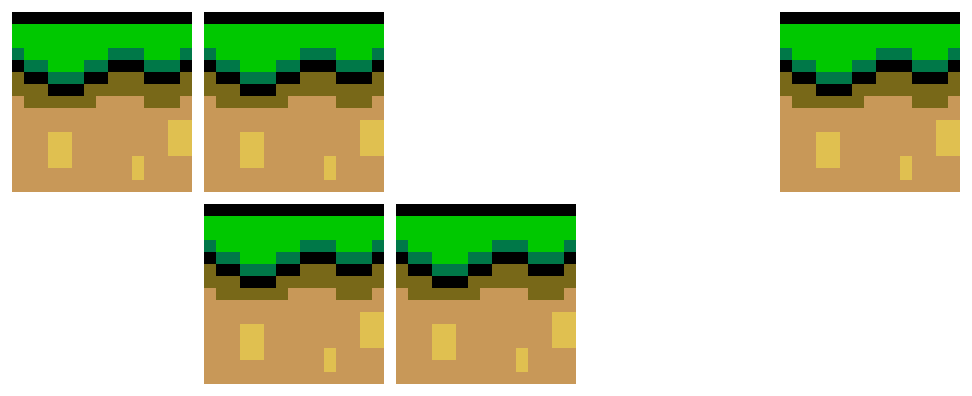
\includegraphics[width=0.5\textwidth]{squash_example.png}
  }\\
  \subfloat[\texttt{squash=false}]{%
    \centering
    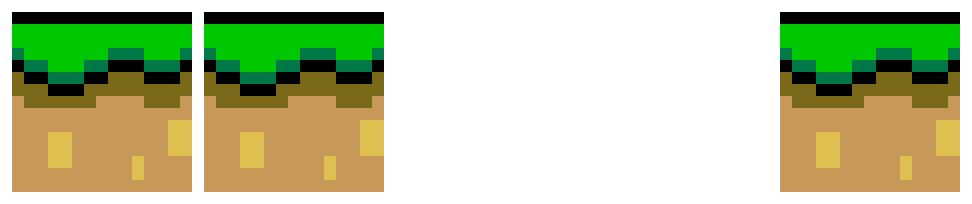
\includegraphics[width=0.5\textwidth]{squash_false.png}
  }\\
  \subfloat[\texttt{squash=true}]{%
    \centering
    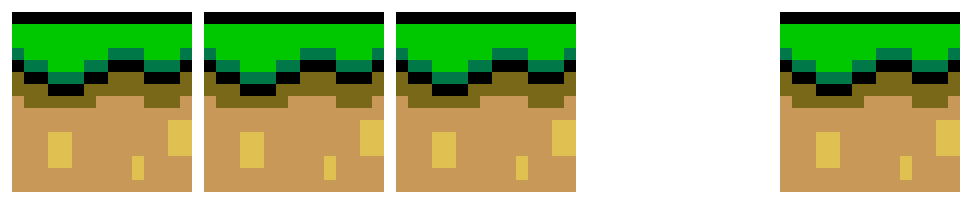
\includegraphics[width=0.5\textwidth]{squash_true.png}
  }%
  \caption{The two ways to obtain 1-dimensional data. Given (a)~as the
    input for either case, the outcome is either (b)~when taking the
    maximum over all rows or (c)~when squashing over all rows.}
  \label{fig:squash-example}
\end{figure}

Each of these can work on any combination of object types of data in
the level; for example, we can have 2-dimensional data containing only
Koopa sprites. Or 3-dimensional data containing only tiles and goal
sprites (as mentioned in the paragraph on layers on
page~\pageref{par:layers}, section~\ref{sec:levels}, we defined a
subset of the object type ``sprite'' containing only sprites directly
relevant to reaching the goal). With this, we can easily test models
on smaller data and adjust towards more complex problems.

For 3-dimensional data it is necessary to provide some information for
each of these combinations so that~-- as mentioned above~-- both data
loaders and models can properly handle different input sizes. \\
This information is the object types the data was created with and the
input size for sequence prediction models and GANs (the input sizes
will be calculated automatically in the future). Our system is easily
extensible to support any desired types; we only implemented the
following (as mentioned, only 3D~data needs extra implementations):
\begin{itemize}
\item \texttt{1d}: any 1-dimensional data
\item \texttt{2d}: any 2-dimensional data
\item \texttt{3dtiles}: 3-dimensional data containing all tile layers
\item \texttt{3d}: 3-dimensional data containing all layers
\end{itemize}
We also provide specific model creation functions for each of these
dimensionalities, giving the user simple access to the correct model
for each task. We will discuss this in detail in
sections~\ref{sec:generation-via-prediction}
and~\ref{sec:first-screen-generation}.

In this thesis, we work with data in column form. This means that our
models read levels column per column from the left to right. We
decided on this order as it captures elements in the past better than
reading the level row per row (where you go back and forth between the
start and end of the level). We also made it possible to read the
levels tile by tile if desired. The order is the same as for the
columns, reading from top to bottom, then from left to right. It is
also possible to change this order to read from bottom to top, then
from left to right. This may improve results at it may be more
important to first analyze the ground before predicting data above.

Now, we will summarize all the simplifications in our data set.

\subsubsection{Simplifications}
\label{sec:simplifications}

We already explained our simplifications in various locations above.
This is a comprehensive list of all of them:
\begin{itemize}
\item Levels are observed independently, meaning no connected levels
  are seen.
\item We omit a lot of metadata. (We suggest the omitted data is not
  related to level generation. As they are already parsed, including
  the omitted data is only a matter of uncommenting and adding a few
  lines of code, adjusting model inputs, and database generation.)
\item Test levels or unfinished levels~-- unless contained in the
  original game~-- are in the dataset.
\item Any data that is out of bounds is ignored (for example, sprites
  may ``fall down'' from a position above level bounds; we ignore
  those).
\item We assume that levels always go from left to right. This is only
  a problem during training as it arbitrarily makes training harder
  (only very few levels go from the right to the left). (We could
  determine whether the main entrance is at the left or right and
  horizontally flip the level accordingly. Even with this
  augmentation, handling levels with a starting position in the middle
  is simply not possible with our architecture.)
\item The type of tile that is assumed to be a level's ground
  (relevant for 1-~and 2-dimensional data generation) is determined
  heuristically (explained above; the first non-empty tile below
  Mario's starting position or tile~256 if none is found).
\item Levels that are (1)~vertical, (2)~boss levels or (3)~levels with
  layer~2 interaction are excluded.
\item Levels with modes deemed unusable by Lunar Magic are excluded.
\item Expanded levels (as designated by Lunar Magic) are excluded.
\item If the database contains a single sprite, we exclude all levels
  without a sprite header.
\end{itemize}

We will now explain our sequence prediction methods in detail.

%%% Local Variables:
%%% mode: latex
%%% TeX-master: "../../SMWLevelGenerator"
%%% End:

